\begin{frame}{Heterogeneous Environment}
  \vspace{1em}
  \begin{figure}
    \centering
    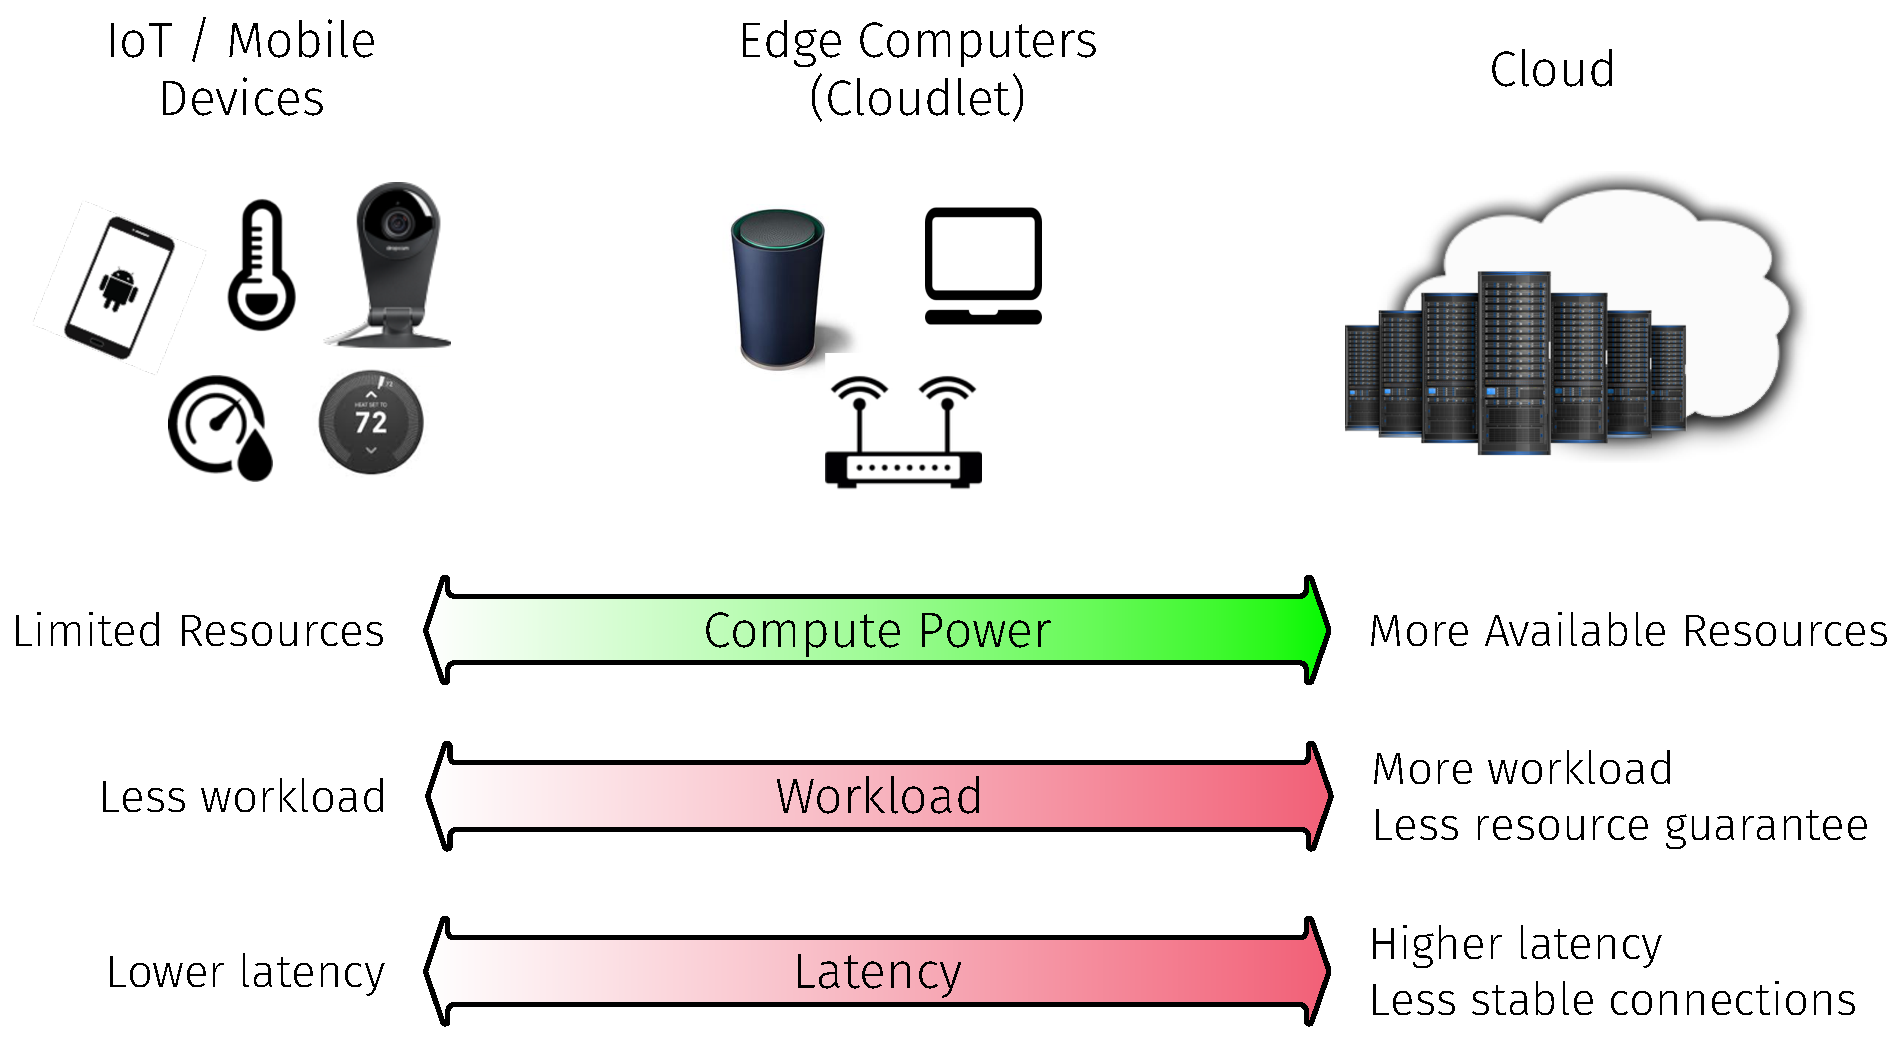
\includegraphics[width=0.95\linewidth]{figures/heterogeneous.pdf}
    \caption{Characteristics of IoT/mobile, edge and cloud}
  \end{figure}
\end{frame}

\begin{frame}{Bayesian Optimization}
  Bayesian optimization provides a principled way for searching optimal
  hyperparameters for a single algorithm. Effective for,
  
  \begin{itemize}
    % https://dhnzl.files.wordpress.com/2016/12/fuzzymad2016_bo_pdf.pdf
    \item Evaluating each sample is expensive.
    \item The objective is a black-box.
    \item The evaluation can be noisy.
  \end{itemize}

  \begin{columns}
    \footnotesize
    \column{0.5\textwidth}
    Gaining attraction for system tuning:

    \begin{itemize}
    \item CherryPick~\cite{alipourfard2017cherrypick}
    \item FLASH~\cite{zhang2016flash}
    \item BOAT~\cite{dalibard2017boat}
    \item Google Cookie\cite{solnik2017bayesian}
    \end{itemize}
    \column{0.5\textwidth}
    \begin{figure}
      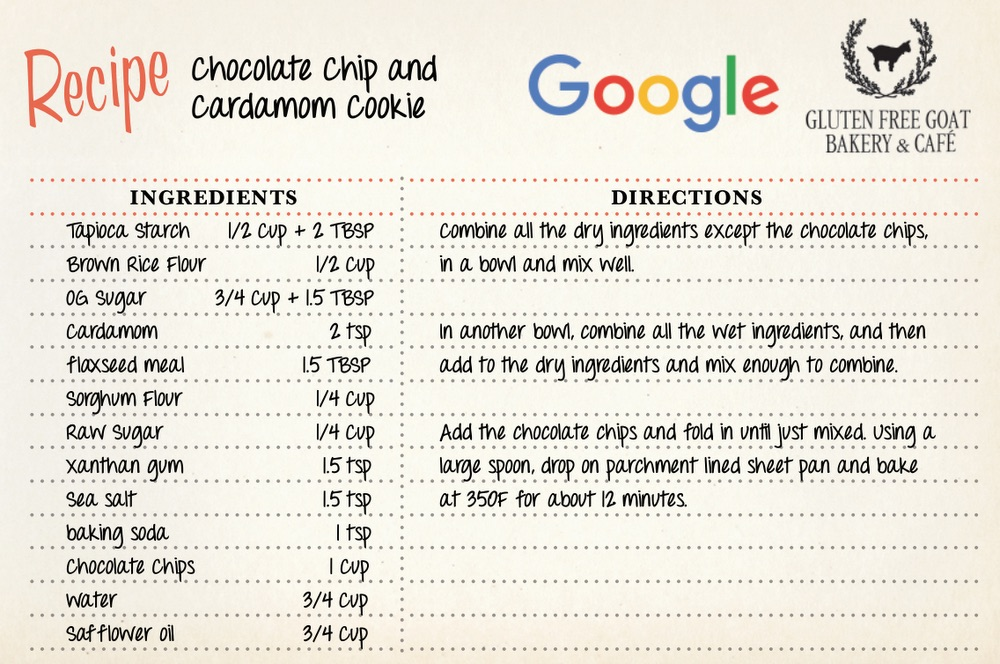
\includegraphics[width=\linewidth]{figures/google-cookie.jpg}
    \end{figure}
  \end{columns}
  
\end{frame}

\begin{frame}{Bayesian Optimization (One Objective)}
  \vspace{1em}
  \begin{figure}
    \centering
    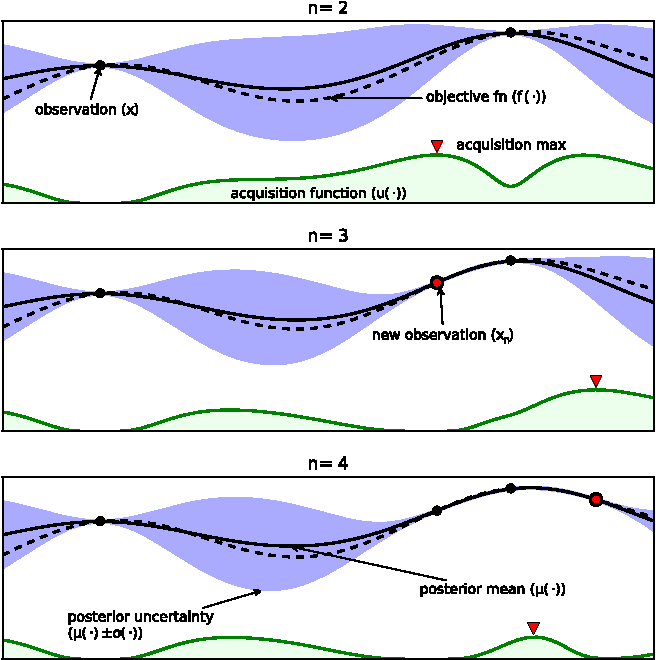
\includegraphics[width=0.5\linewidth]{figures/serving-bo-illustration.pdf}
    \caption{\cite{shahriari2016taking}}
  \end{figure}
\end{frame}

\begin{frame}{Bayesian Optimization (Two Objectives)}
  \vspace{1em}
  \begin{figure}
    \centering
    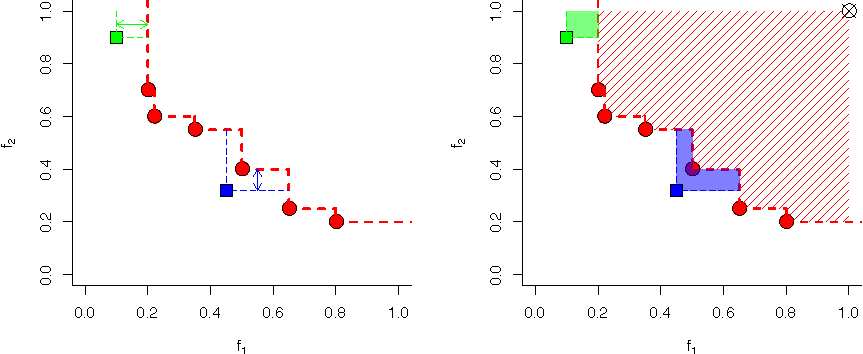
\includegraphics[width=0.95\linewidth]{figures/serving-bo-2d}
    \caption{\cite{binoisgpareto}}
  \end{figure}
\end{frame}

\begin{frame}{Exhaustive}
  \vspace{1em}
  \begin{figure}
    \centering
    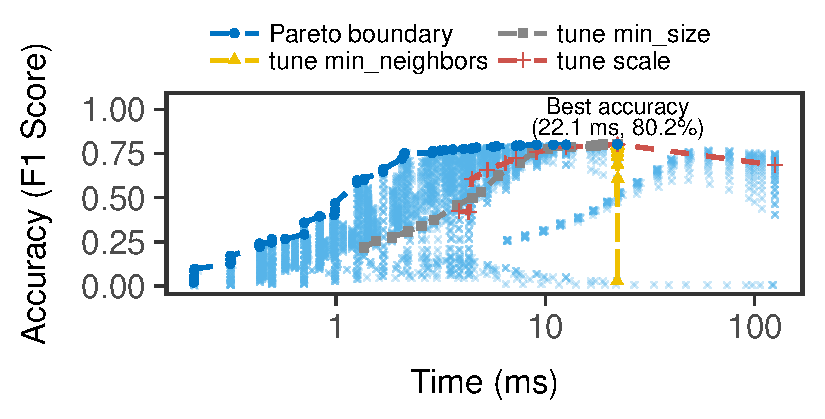
\includegraphics[width=0.95\linewidth]{figures/serving-eval-exhaustive.pdf}
  \end{figure}
\end{frame}

\begin{frame}{Bayesian Optimization}
  \vspace{1em}
  \begin{figure}
    \centering
    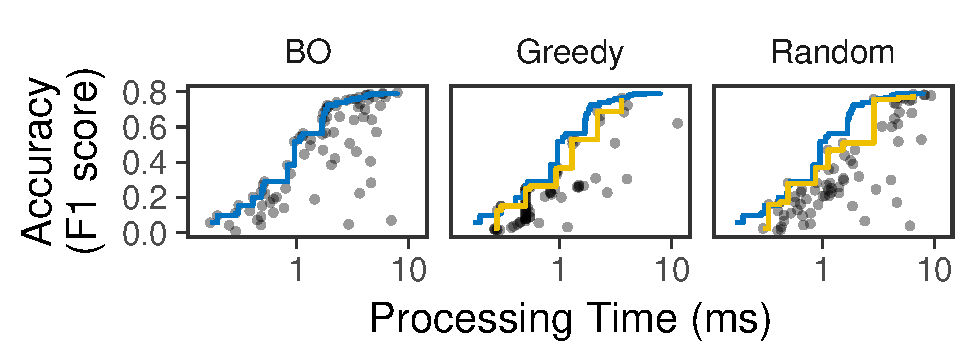
\includegraphics[width=0.95\linewidth]{figures/serving-eval-bo.pdf}
    \caption{BO evaluates 50 configurations and recommends 29 configurations as
      the Pareto-optimal boundary (the blue line). Greedy and Random find
      sub-optimal Pareto configurations with a budget of 80 evaluations (the
      yellow line in each figure).}
  \end{figure}
\end{frame}

%%% Local Variables:
%%% mode: latex
%%% TeX-master: "../talk"
%%% TeX-engine: xetex
%%% End:
